\documentclass[25pt, a0papper, portrait]{tikzposter}
\usepackage[utf8]{inputenc}
\usepackage{xcolor}
\usepackage{graphicx,mwe}
\usepackage{filecontents}% http://ctan.org/pkg/filecontents
\usepackage{lipsum}% http://ctan.org/pkg/lipsum
\usepackage{tikz}
\usepackage{multicol}
\usepackage{adjustbox}

\makeatletter
\def\TP@titlegraphictotitledistance{-9cm}
\settitle{ \centering \vbox{
		\@titlegraphic \\ [\TP@titlegraphictotitledistance] 
		\centering
		\color{titlefgcolor} {\bfseries \Huge \sc \@title \par}
		\vspace*{1em}
		{\huge \@author \par} \vspace*{1em} {\LARGE \@institute}
	}}
\makeatother
 
\title{TCPSnitch: Dissecting the Socket API Usage}
\author{\textbf{Gregory Vander Schueren}, Quentin De Coninck, Olivier Bonaventure \\ \texttt{gregory.vanderschueren@tessares.net} \\ \texttt{https://tcpsnitch.org}}
\date{\today}
\titlegraphic{
	
\includegraphics[width=0.06\textwidth]{figures/UCL}
    \hfill

\includegraphics[width=0.15\textwidth]{figures/tessares}
}

\institute{Université catholique de Louvain, Louvain-la-Neuve, Belgium}
 
\usepackage{blindtext}
\usepackage{comment}
\renewcommand*\familydefault{\sfdefault}
\usepackage[T1]{fontenc}
 
\usetheme{Desert}
\usenotestyle{Sticky}

\usepackage[backend=bibtex]{biblatex}
\addbibresource{biblio.bib,2011.bib}

\tikzposterlatexaffectionproofoff
\begin{document}
\maketitle

%{%<--------- Start scope
	\colorlet{notebgcolor}{yellow} %<---- change color
	%\block{BlocktitleB}{\lipsum[2]}
%}%<--------- End scope

% FIRST ROW
\begin{columns}
    \column{0.50}
    \block{Methodology}{
        lalala
        \vspace{5cm}
    }
    \column{0.50}
    \block{TCPSnitch}{
        \begin{itemize}
            \item Command-line application that collects detailed traces of the
        interactions between networked applications and the TCP/IP stack.
            \item Intercepts function calls and collects parameters,
            return value, timestamps, the thread id, the error number, etc.
            \item Runs on Linux and Android.
            \item Open-source \url{https://github.com/GregoryVds/tcpsnitch}.
        \end{itemize}
    }
\end{columns}


% SECOND ROW
\begin{columns}
    \column{0.50}
    \block{Dataset}{
        lalala
        \vspace{5cm}
    }
    \column{0.50}
    \block{https://tcpsnitch.org}{
        \begin{itemize}
            \item TCPSnitch automatically uploads traces to \url{https://tcpsnitch.org}.
            \item Public platform designed to centralize and visualize the traces.
            \item Upon uploading a trace, multiple metrics and charts are computed.
            \item Open-source \url{https://github.com/GregoryVds/tcpsnitch_web}.
        \end{itemize}
        \begin{tikzfigure}
            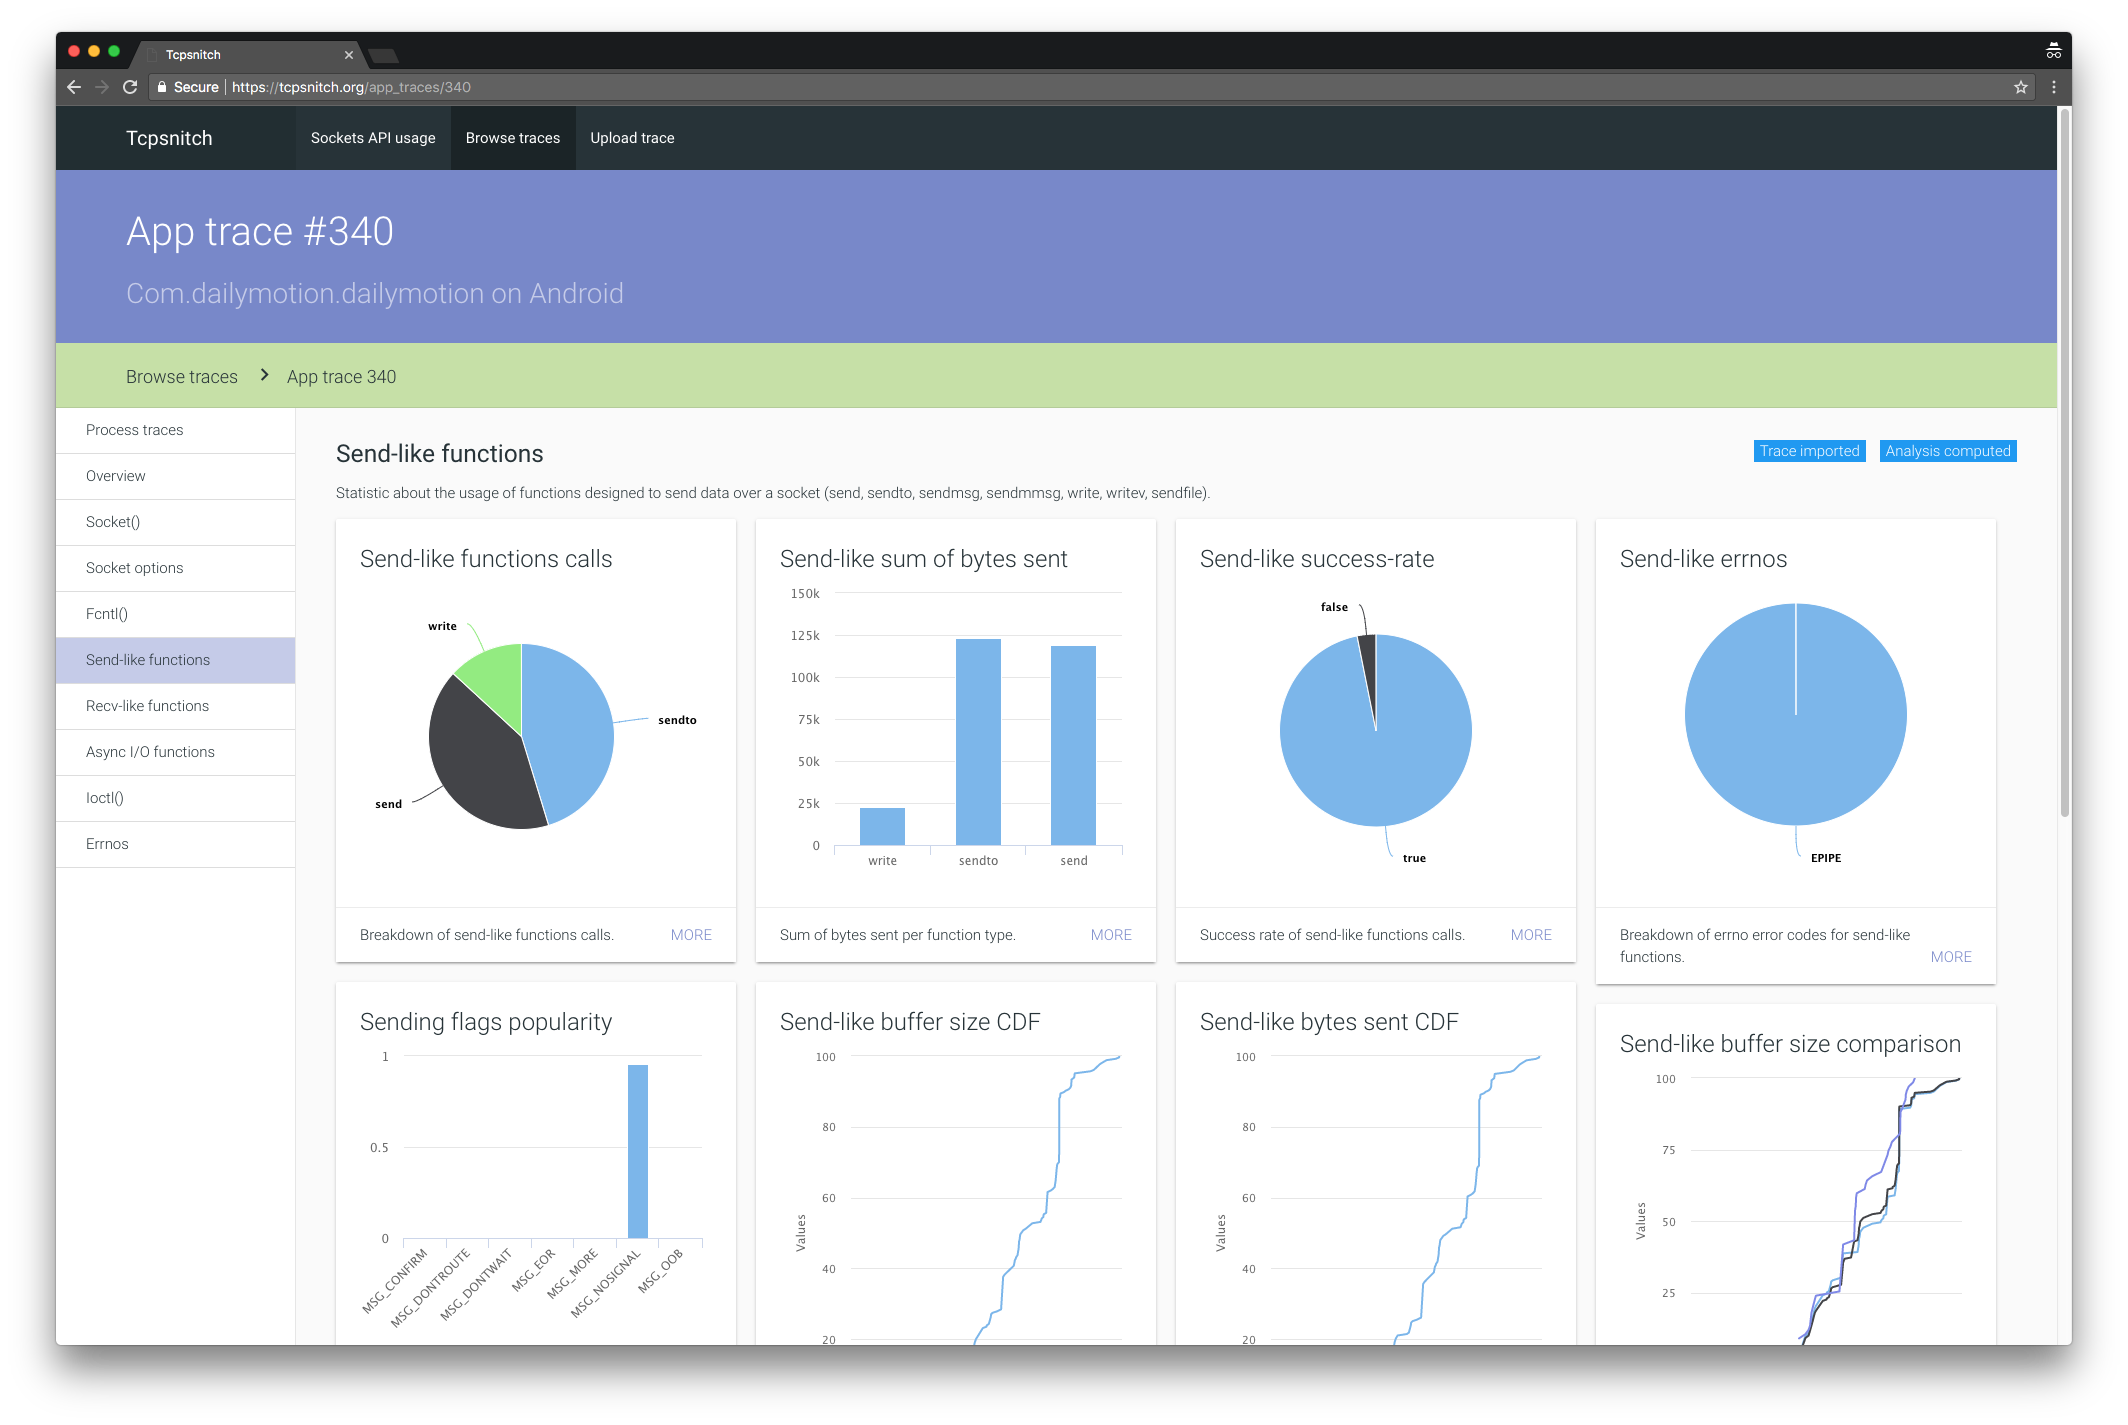
\includegraphics[width=.4\textwidth]{figures/org2}
        \end{tikzfigure}
    }
\end{columns}



% THRID ROW
\begin{columns}
    \column{0.50}
    \block{API usage on Linux and Android differ greatly}{
        \begin{tikzfigure}
           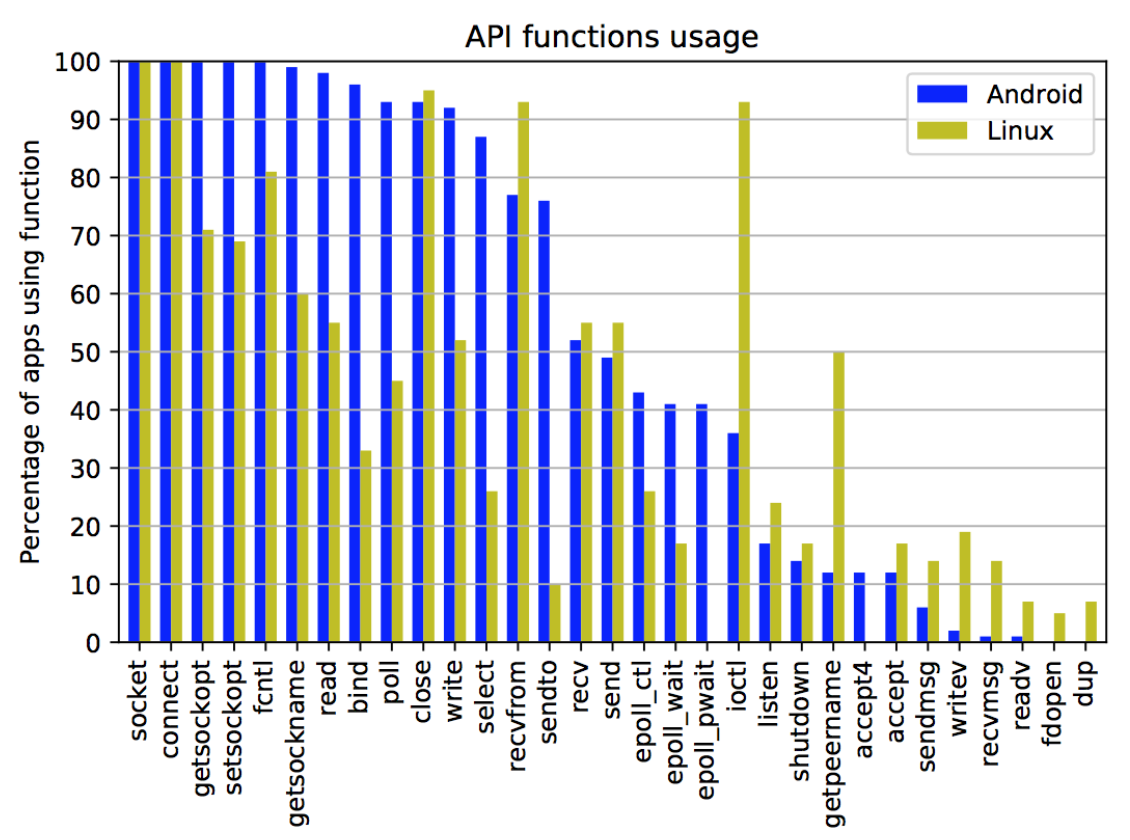
\includegraphics{figures/finding1}
        \end{tikzfigure}
    }
    \column{0.50}
    \block{API usage driven by high-level frameworks and libraries}{

    An HTTP GET request over TLS yields different API footprints with different libraries\\
\begin{tikzfigure}
\begin{tabular}{lllllll}
\hline
\textbf{Language}   & Ruby        & Python   & JavaScript        & Perl        & PHP\\ \hline
\textbf{Library}        & \texttt{Net:HTTP} & \texttt{urllib2}  & \texttt{https mod}  & \texttt{LWP::Simple} & \texttt{f\_g\_contents} \\ \hline
\textbf{API calls}  & 186         & 353      & 106               & 465         & 920\\ \hline
\textbf{Bytes recv} & 65~KB       & 175~KB   & 175~KB            & 178~KB      & 175~KB\\ \hline
\textbf{Main API call}  & \texttt{read()}      & \texttt{read()}   & \texttt{read()} & \texttt{read()}      & \texttt{fcntl()} \\ \hline
\textbf{Socket option}  & \texttt{TCP\_NODELAY} & \texttt{SO\_TYPE} & \texttt{SO\_ERROR} & \texttt{SO\_ERROR} & \texttt{SO\_ERROR}\\ \hline
\textbf{Async I/O}      & \texttt{ppoll()} & N/A      & N/A  &  \texttt{select()} & \texttt{poll()} \\ \hline
\end{tabular}
\end{tikzfigure}

        \vspace{5cm}
    }
\end{columns}


% FOURTH ROW
\begin{columns}
    \column{0.33}
    \block{Android: API usage differs from textbook usage}{
        \begin{tikzfigure}
           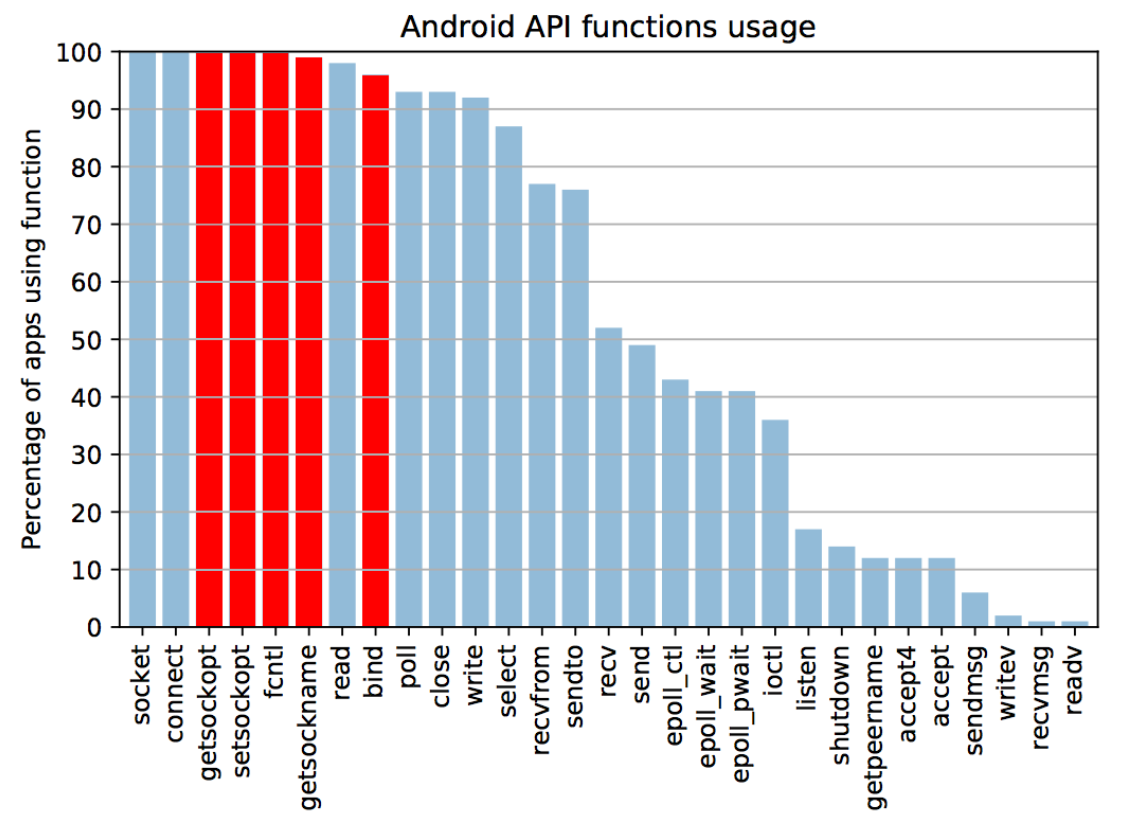
\includegraphics{figures/finding3}
        \end{tikzfigure}
    }
    \column{0.33}
    \block{Android: UDP sockets usage} {
        On Android, UDP sockets are mainly used as a shortcut to retrieve
        information about the network configuration.
        \begin{tikzfigure}
           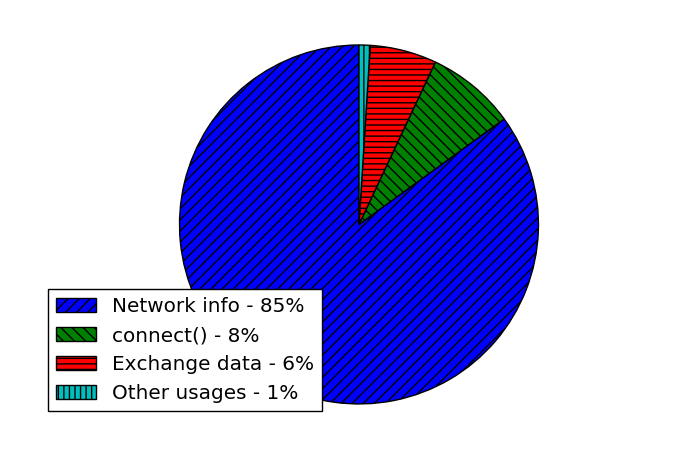
\includegraphics{figures/finding4}
        \end{tikzfigure}
    }
    \column{0.33}
    \block{Android: TCP\_INFO widely used}{
        For Facebook applications, the number of TCP\_INFO calls seems to be
        a linear function of the number of recv() calls.
        \begin{tikzfigure}
           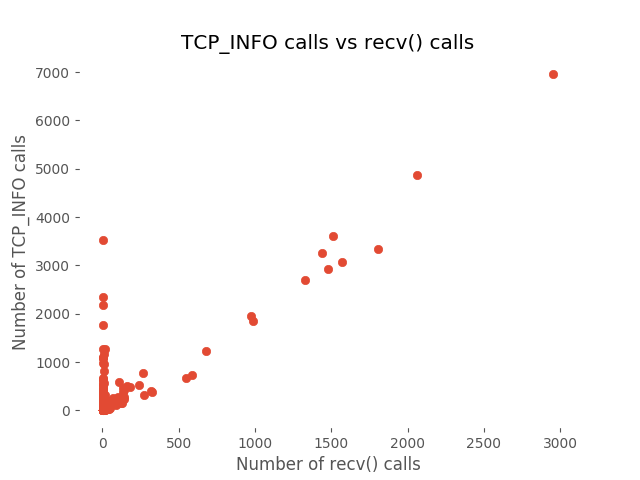
\includegraphics{figures/finding5}
        \end{tikzfigure}
    }
\end{columns}

\end{document}
